\chapter{Práctica 4}
\begin{figure}[h]
  \begin{center}
    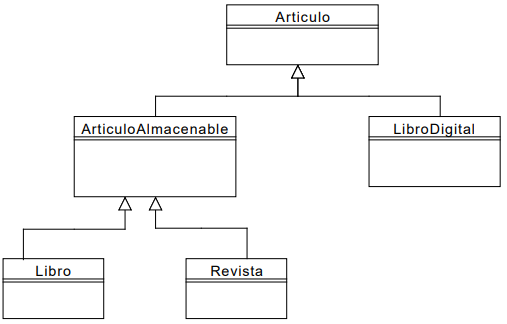
\includegraphics[width=\textwidth]{Pics/P4_1.png}
  \end{center}
  \caption{Diagrama de clases de la práctica 4.}
\end{figure}

Esta es la última práctica, y se corresponde con el tema de polimorismo.

Como vemos en el diagrama la clase Articulo se especializa en dos subclases, debido a esto vamos a tener que realizar ciertas modificaciones en dicha clase.
\section{Modificación de la clase Articulo}
La clase Articulo la vamos a declarar ahora como una clase abstracta, es decir, no se pueden crear objetos de ella ya que tiene un método definido como virtual puro, ese método será:
\begin{center}
  \begin{verbatim}
    virtual void impresion_especifica(std::ostream&)const = 0;
  \end{verbatim}
\end{center}

El constructor de Articulo también sufre cambios, siendo ahora el primer parámetro del mismo una referencia constante a un conjunto de Autores de una nueva clase llamada \texttt{Autor}.

El atributo \texttt{stock\_} deja de pertencer a la clase Articulo, y ahora pertenece a la clase ArticuloAlmacenable, por tanto, los observadores del atributo también se pasan a la clase ArticuloAlmacenable, el resto de los parámetros son referencia, titulo, fecha de publicación y el precio del articulo.

Vamos a definir una clase de excepcion \textbf{Articulo::Autores\_vacios}, ya que un Articulo tiene que tener como mínimo un Autor.


El método \texttt{impresion\_especifica()} (`comentado previamente'), realizará modificaciones en el método \texttt{mostrar\_carro()} por tanto, tenemos que reescribir esa función para que no dependa del operador de inserción de Articulo y conserve el formato de salida original.

El formato de salida del método será:
\begin{itemize}
  \item Libros:
  \begin{center}
    \begin{verbatim}
    [103] "Brácula, el no vivo", de Echo, Rey. 1902. 39,95 €
    455 págs., 4 unidades.
    \end{verbatim}
  \end{center}
  \item Revistas:
  \begin{center}
    \begin{verbatim}
    [701] "Byter", de Verde. 2022. 15,70 €
    Número: 101, Periodicidad: 30 días.
    Próximo número a partir de: miércoles 14 de septiembre de 2022.
    \end{verbatim}
  \end{center}
  \item LibrosDigitales:
  \begin{center}
    \begin{verbatim}
    [036] "55 días en Pasquín", de Fuertes. 2007. 12,00 €
    A la venta hasta el martes 30 de septiembre de 2008.
    \end{verbatim}
  \end{center}
\end{itemize}

\section{Clase Autor}
Como hemos comentado en la modificación de la clase Articulo, esta recibe como parámetro una referencia constante de un Autor.

Esta clase Autor contiene los datos de los autores (nombre, apellido y dirección), donde no contemplamos ninguna excepción.

Además contendrá observadores correspondientes a los atributos llamados \texttt{nombre()},\\\texttt{apellidos()} y \texttt{direccion()}, que devuelven una referencia constante de la Cadena.
\newpage
\section{La subclase ArticuloAlmacenable}
Esta clase al igual que Articulo será una clasa abstracta ya que también contiene el método:
\begin{center}
  \begin{verbatim}
    virtual void impresion_especifica(std::ostream&)const = 0;
  \end{verbatim}
\end{center}

Esta clase almacena el atributo \texttt{stock} que previamente pertenecía a la clase Articulo, ya que como bien dice su nombre, un ArticuloAlmacenable debe de ser un Articulo que se pueda almacenar, es decir, que tiene un stock.

Podemos consultar el stock de un ArticuloAlmacenable mediante el observador \texttt{stock()} y su sobrecarga para modificarlo.

Como esta clase es una especialización de Articulo, ArticuloAlmacenable en su constructor tendrá que recibir todos los atributos con los que se inicializa un Articulo más el stock propio del ArticuloAlmacenable.

\section{La subclase LibroDigital}
Es una clase derivada de la clase Articulo, debido a que no tenemos que almacenar el número de ejemplares de los mismos.

Tenemos que tener en cuenta la fecha de expiración(\texttt{f\_expir()}) donde los ebooks dejan de venderse.

Esta fecha no se puede modificar una vez se cree el objeto y se va a crear con los mismos parámetros que la clase artículo más el atributo propio de la fecha de expiración.

Si la fecha de expiración es menor a la del Pedido no se podrá comprar. Para que esto se cumpla tendremos que modificar el constructor de la clase Pedido si un *Usuario* ha introducido un *LibroDigital* expirado, es decir, este no se añadirá al pedido.

Si el Pedido que vacío por este motivo, se lanzará la excepción \textbf{Pedido::Vacio}.

\section{La subclase Libro}
Esta clase es una derivación de la clase de ArticuloAlmacenable, o sea, que tiene también un stock asociado, además que tiene como atributo propio el número de paginas de cada objeto libro.

Podemos consultar el número de páginas (que es no modificable) mediante el observador \texttt{\_pag()}.

El constructor de Libro tiene los mismo parámetros que ArticuloAlmacenable pero añadiendole el atributo propio del número de páginas, que por defecto es 0.

\section{La subclase Revista}

También es una clase que contiene un stock, por tanto, es derivada de la clase ArticuloAlmacenable.

Tenemos un numero con el observador \texttt{numero()} y la periodicidad con el observador \texttt{periodicida()}. No se pueden modificar ninguno de los dos cuando se cree el objeto.

\section{Modificación clase Articulo.hpp}
\begin{minted}[breaklines]{C++}
  #ifndef ARTICULO_HPP
#define ARTICULO_HPP

// Inclusión de librerías
#include "../P1/fecha.hpp"
#include "../P1/cadena.hpp"
#include <iostream>
#include <iomanip>
#include <locale.h>
#include <set>

/*-----Clase Autor de la P4-----*/
class Autor{
public:
  // No definimos la relación con Articulo aqui ya que no
  // nos hace falta.
  Autor(const Cadena &nombre, const Cadena &apellido, const Cadena &direccion)
      : nom_(nombre), apell_(apellido), dir_(direccion) {}
  // Consultores de la clase
  inline const Cadena &nombre() const noexcept { return nom_; }
  inline const Cadena &apellidos() const noexcept { return apell_; }
  inline const Cadena &direccion() const noexcept { return dir_; }

private:
  Cadena nom_, apell_, dir_;
};

/*-----Clase Aticulo de la P4-----*/
class Articulo{
public:
  /*-----Relación entre Articulo - Autor-----*/
  // podemos definirlo como una asociación o agregación, que cada Articulo contendrá
  // un conjunto de Autores.
  typedef std::set<Autor *> Autores;

  // Como un Articulo puede tener como mínimo 1 autor y además sin autor no hay articulo
  Articulo(const Autores &autores, Cadena referencia, Cadena titulo,
           Fecha f_publi, double precio);

  // Observadores de la clase
  inline const Cadena &referencia() const noexcept { return referencia_; }
  inline const Cadena &titulo() const noexcept { return titulo_; }
  inline const Fecha &f_publi() const noexcept { return fpubli_; }
  inline double precio() const noexcept { return precio_; }
  inline double &precio() noexcept { return precio_; }
  // Desaparece en esta práctica
  //  inline unsigned stock()const noexcept{return stock_;}
  //  inline unsigned& stock()noexcept{return stock_;}
  inline const Autores &autores() const noexcept { return autores_; }
  // Exepcion de la clase
  class Autores_vacios{
  };

  // Nuevo operador de inserción en flujo
  virtual void impresion_especifica(std::ostream &) const = 0;

  // Como esta clase se va a especializar en otras su destructor debe de ser
  // virtual para que puedan llamarse a los destructores de las clases derivadas
  virtual ~Articulo() = default;

private:
  Autores autores_; // relación de las clases Articulo - Autor
  const Cadena referencia_, titulo_;
  const Fecha fpubli_;
  double precio_;
  // unsigned stock_; Desaparece en esta práctica
};

// Operador de inserción en flujo
std::ostream &operator<<(std::ostream &, const Articulo &) noexcept;

/*-----Clase Derivada ArticuloAlamacenable-----*/
class ArticuloAlmacenable : public Articulo{
  public:
    ArticuloAlmacenable(const Autores &autores, Cadena referencia, Cadena titulo,
                        Fecha f_publi, double precio, unsigned stock = 0)
        : Articulo(autores, referencia, titulo, f_publi, precio), stock_(stock) {}

    // Observadores de la clase
    inline unsigned stock() const noexcept { return stock_; }
    inline unsigned &stock() noexcept { return stock_; }

  protected: // se pone protected para que las clases derivadas de esta puedan hacer uso del atributo
    // Atributo de la clase Articulo que lo define
    unsigned stock_;
};

/*-----Clase Derivada Libro-----*/
class Libro final : public ArticuloAlmacenable{
  public:
    Libro(const Autores &autores, Cadena referencia, Cadena titulo,
          Fecha f_publi, double precio, unsigned paginas = 0, unsigned stock = 0) : ArticuloAlmacenable(autores, referencia, titulo, f_publi, precio, stock), n_pag_(paginas) {}
    // Observadores de la clase
    inline const unsigned &n_pag() const noexcept { return n_pag_; }
    // Método virtual heredado
    void impresion_especifica(std::ostream &) const override final;

  private:
    // Atributo de la clase que lo define
    const unsigned n_pag_;
};

/*-----Clase Derivada Revista-----*/
class Revista final : public ArticuloAlmacenable{
public:
    Revista(const Autores &autores, Cadena referencia, Cadena titulo,
            Fecha f_publi, double precio, const unsigned numero, const unsigned f, unsigned stock = 0) : ArticuloAlmacenable(autores, referencia, titulo, f_publi, precio, stock), numero_(numero), periodicidad_(f) {}
    // Observadores de la clase
    inline unsigned numero() const noexcept { return numero_; }
    inline unsigned periodicidad() const noexcept { return periodicidad_; }
    // Método virtual heredado
    void impresion_especifica(std::ostream &) const override final;

  private:
    const unsigned numero_, periodicidad_;
};

/*-----Clase Derivada LibroDigital-----*/
class LibroDigital final : public Articulo{
  public:
    LibroDigital(const Autores &autores, Cadena referencia, Cadena titulo,
                Fecha f_publi, double precio, const Fecha &f_expir) : Articulo(autores, referencia, titulo, f_publi, precio), f_expir_(f_expir) {}
    // Observador de la clase
    inline const Fecha &f_expir() const noexcept { return f_expir_; }
    // Método virtual heredado
    void impresion_especifica(std::ostream &) const override final;

  private:
    const Fecha f_expir_;
};

#endif // !ARTICULO_HPP
\end{minted}
\section{Modificación clase Articulo.cpp}
\begin{minted}[breaklines]{C++}
#include "articulo.hpp"
/*-----Implementación de la clase Articulo-----*/
Articulo::Articulo(const Autores &autor, Cadena referencia, Cadena titulo, Fecha f_publi, double precio) :
   autores_(autor), referencia_(referencia), titulo_(titulo), fpubli_(f_publi), precio_(precio){
  // Lo unico que tenemos que comprobar que dicho articulo tenga como mínimo un autor
  if (autores_.empty()) throw Autores_vacios();
}

// Operador de inserción en flujo
std::ostream &operator<<(std::ostream &output, const Articulo &art) noexcept{
  std::locale::global(std::locale(""));
  output << "[" << art.referencia() << "] " << "\"" << art.titulo() << "\"" << ", de ";
  // recorremos el conjunto de autores del articulo
  auto i = art.autores().begin();
  output << (*i)->apellidos();
  for (i++; i != art.autores().end(); i++){
    output << ", " << (*i)->apellidos();
  }
  output << ". " << art.f_publi().anno() << ". "
         << std::fixed << std::setprecision(2) << art.precio() << " €" << std::endl
         << "\t";
  // llamamos al método heredado.
  art.impresion_especifica(output);
  return output;
}
/*-----Implementación del Método virtual-----*/
void Libro::impresion_especifica(std::ostream &output) const{
  output << n_pag_ << " págs., " << stock_ << " unidades.";
}
void Revista::impresion_especifica(std::ostream &output) const{
  output << "Número: " << numero_ << ", Periodicidad: " << periodicidad_ << " días."
    << "\n"<< "\t"<< "Próximo número a partir de: " << Fecha(f_publi() + periodicidad_) << ".";
}
void LibroDigital::impresion_especifica(std::ostream &output) const{
  output << "A la venta hasta el " << f_expir_ << ".";
}
\end{minted}
\section{Modificación clase Pedido.cpp}
Como la clase Articulo ya no tiene más el atrbuto stock, a la hora de comprarlo en el constructor de la clase Pedido, tenemos que realizar una conversión explicita de Articulo ya sea a ArticuloAlmacenable.

También tendremos que comprobar la fecha de expiración de los LibrosDigitales, por lo que también tendremos que realizar una conversión explicita de Articulo a LibroDigital.

Tenemos que hacer esto debido a que la clase Pedido trabaja con un conjunto de Articulos.

\begin{minted}[breaklines]{C++}
Pedido::Pedido(Usuario_Pedido &up, Pedido_Articulo &pa, Usuario &u,const Tarjeta &t, const Fecha &f)
  : num_(n_pedidos_ + 1), tarjeta_(&t), f_pedido_(f), importe_Total_(0.0){
  // Vamos a comprobar todas la excepciones del constructor de pedido
  // Si el usuario no tiene una compra realizada, el pedido está vacio
  if (u.compra().empty()) throw Pedido::Vacio(&u);

  // Si el usuario es otro al que realiza la compra, excepción
  if (t.titular() != &u)  throw Pedido::Impostor(&u);

  // Si la tarjeta está caducada o desactivada, excepción
  if (t.caducidad() < f_pedido_)  throw Tarjeta::Caducada(t.caducidad());

  if (!t.activa())  throw Tarjeta::Desactivada();
  // Si no hay stock del articulo, excepcion.
  // Hacemos la conversión primero y luego comprobamos
  Usuario::Articulos carrito = u.compra();
  for (auto i : carrito){ // carrito del usuario
    if (ArticuloAlmacenable *AA = dynamic_cast<ArticuloAlmacenable *>(i.first)){ // hacemos conversion
      // comprobamos el stock
      if (AA->stock() < i.second){
        u.vaciar_carro();
        throw Pedido::SinStock(AA);
      }
    }
    else if (LibroDigital *LD = dynamic_cast<LibroDigital *>(i.first)){
      // Si la fecha de expiración es < a la fecha del pedido, se añade con cantidad 0
      if (LD->f_expir() < Fecha()){                   // Ha expirado
        u.compra(*LD, 0); // Añadimos al pedido dicho articulo pero con la cantidad a 0
      }
    }
    else throw std::logic_error("Pedido::Pedido - Tipo de articulo no conocido");
  }
  // Comprobamos que no se quede vacio el Pedido
  if (u.compra().empty()) throw Pedido::Vacio(&u);
  // Realizamos la asociación Usuario - Pedido
  up.asocia(*this, u);

  // Vamos a pedir el articulo
  for (auto &i : u.compra()){
    importe_Total_ += i.first->precio() * i.second;
    pa.pedir(*this, *(i.first), i.first->precio(), i.second);

    // Ahora para restar el stock de dicho articulo hacemos lo mismo que arriba
    if (ArticuloAlmacenable *AA = dynamic_cast<ArticuloAlmacenable *>(i.first)){
      AA->stock() -= i.second;
    }
  }
  // Aumentamos el numero de pedidos y vaciamos el carro del usuario
  u.vaciar_carro();
  n_pedidos_++;
}
\end{minted}